\documentclass{article}
\usepackage[margin=1in, paperwidth=8.5in, paperheight=11in]{geometry}
\usepackage{caption}
\usepackage{subcaption}
\usepackage{float}
\usepackage{graphicx}
\usepackage[utf8]{inputenc}
\usepackage[english]{babel}
\usepackage{mathtools}
\usepackage{gensymb}
\usepackage{amstext}
\usepackage{amsmath}
\usepackage{graphicx}
\usepackage{textcomp}
\usepackage{varioref}
\usepackage{fancyref}
\usepackage{subcaption}
\usepackage{comment}
\usepackage{hyperref}
\usepackage{epstopdf}
\usepackage{gensymb}
\usepackage{listings}
\usepackage{xcolor}
\usepackage{listings}
\usepackage{pdfpages}
\usepackage{graphicx}
\usepackage{wrapfig}
\usepackage{lscape}
\usepackage{rotating}
\usepackage{epstopdf}
\usepackage{fancyhdr}
\usepackage{amssymb}
\usepackage{fancyhdr}
\usepackage{soul}
\usepackage{chngcntr}
%font
\usepackage{lmodern}
\usepackage[sfdefault, light]{roboto}

% Document Setup
\pagenumbering{roman}
\pagestyle{fancy}
\addto\captionsenglish{\renewcommand*\contentsname{Table of Contents}}
\DeclareRobustCommand{\hlr}[1]{{\sethlcolor{red}\hl{#1}}}
\graphicspath{{img/}}
\counterwithin{table}{section} %number tables with section#.table#

\begin{document}

\renewcommand{\headrulewidth}{0pt}
\lhead{Olin College of Engineering, E238}
\chead{}
\rhead{} %\rightmark
\lfoot{2017 Formula SAE Electric}
\cfoot{
\includegraphics[width=3cm]{logo_blue.png}}
\rfoot{\thepage}

\begin{titlepage}

    \centering
    \vfill
    
\includegraphics[width=10cm]{logo_blue.png}

    {\bfseries\Large
        \vskip3cm
        Electrical System Form FSAE-E 2017\\
        Car E238\\
    }

    \begin{table}[H]
        \centering
        \label{my-label}
        \begin{tabular}{lr}
        University Name: & Olin College of Engineering \\ \hline
        Team Name: & Olin Electric Motorsports \\ \hline
        Car Number: & E238 \\ \hline
        ESF Contact: & Alex Hoppe \\ \hline
        e-mail: & Alexander.Hoppe@students.olin.edu \\ \hline
        \end{tabular}
    \end{table}
\vfill

\begin{figure}[H]
\centering
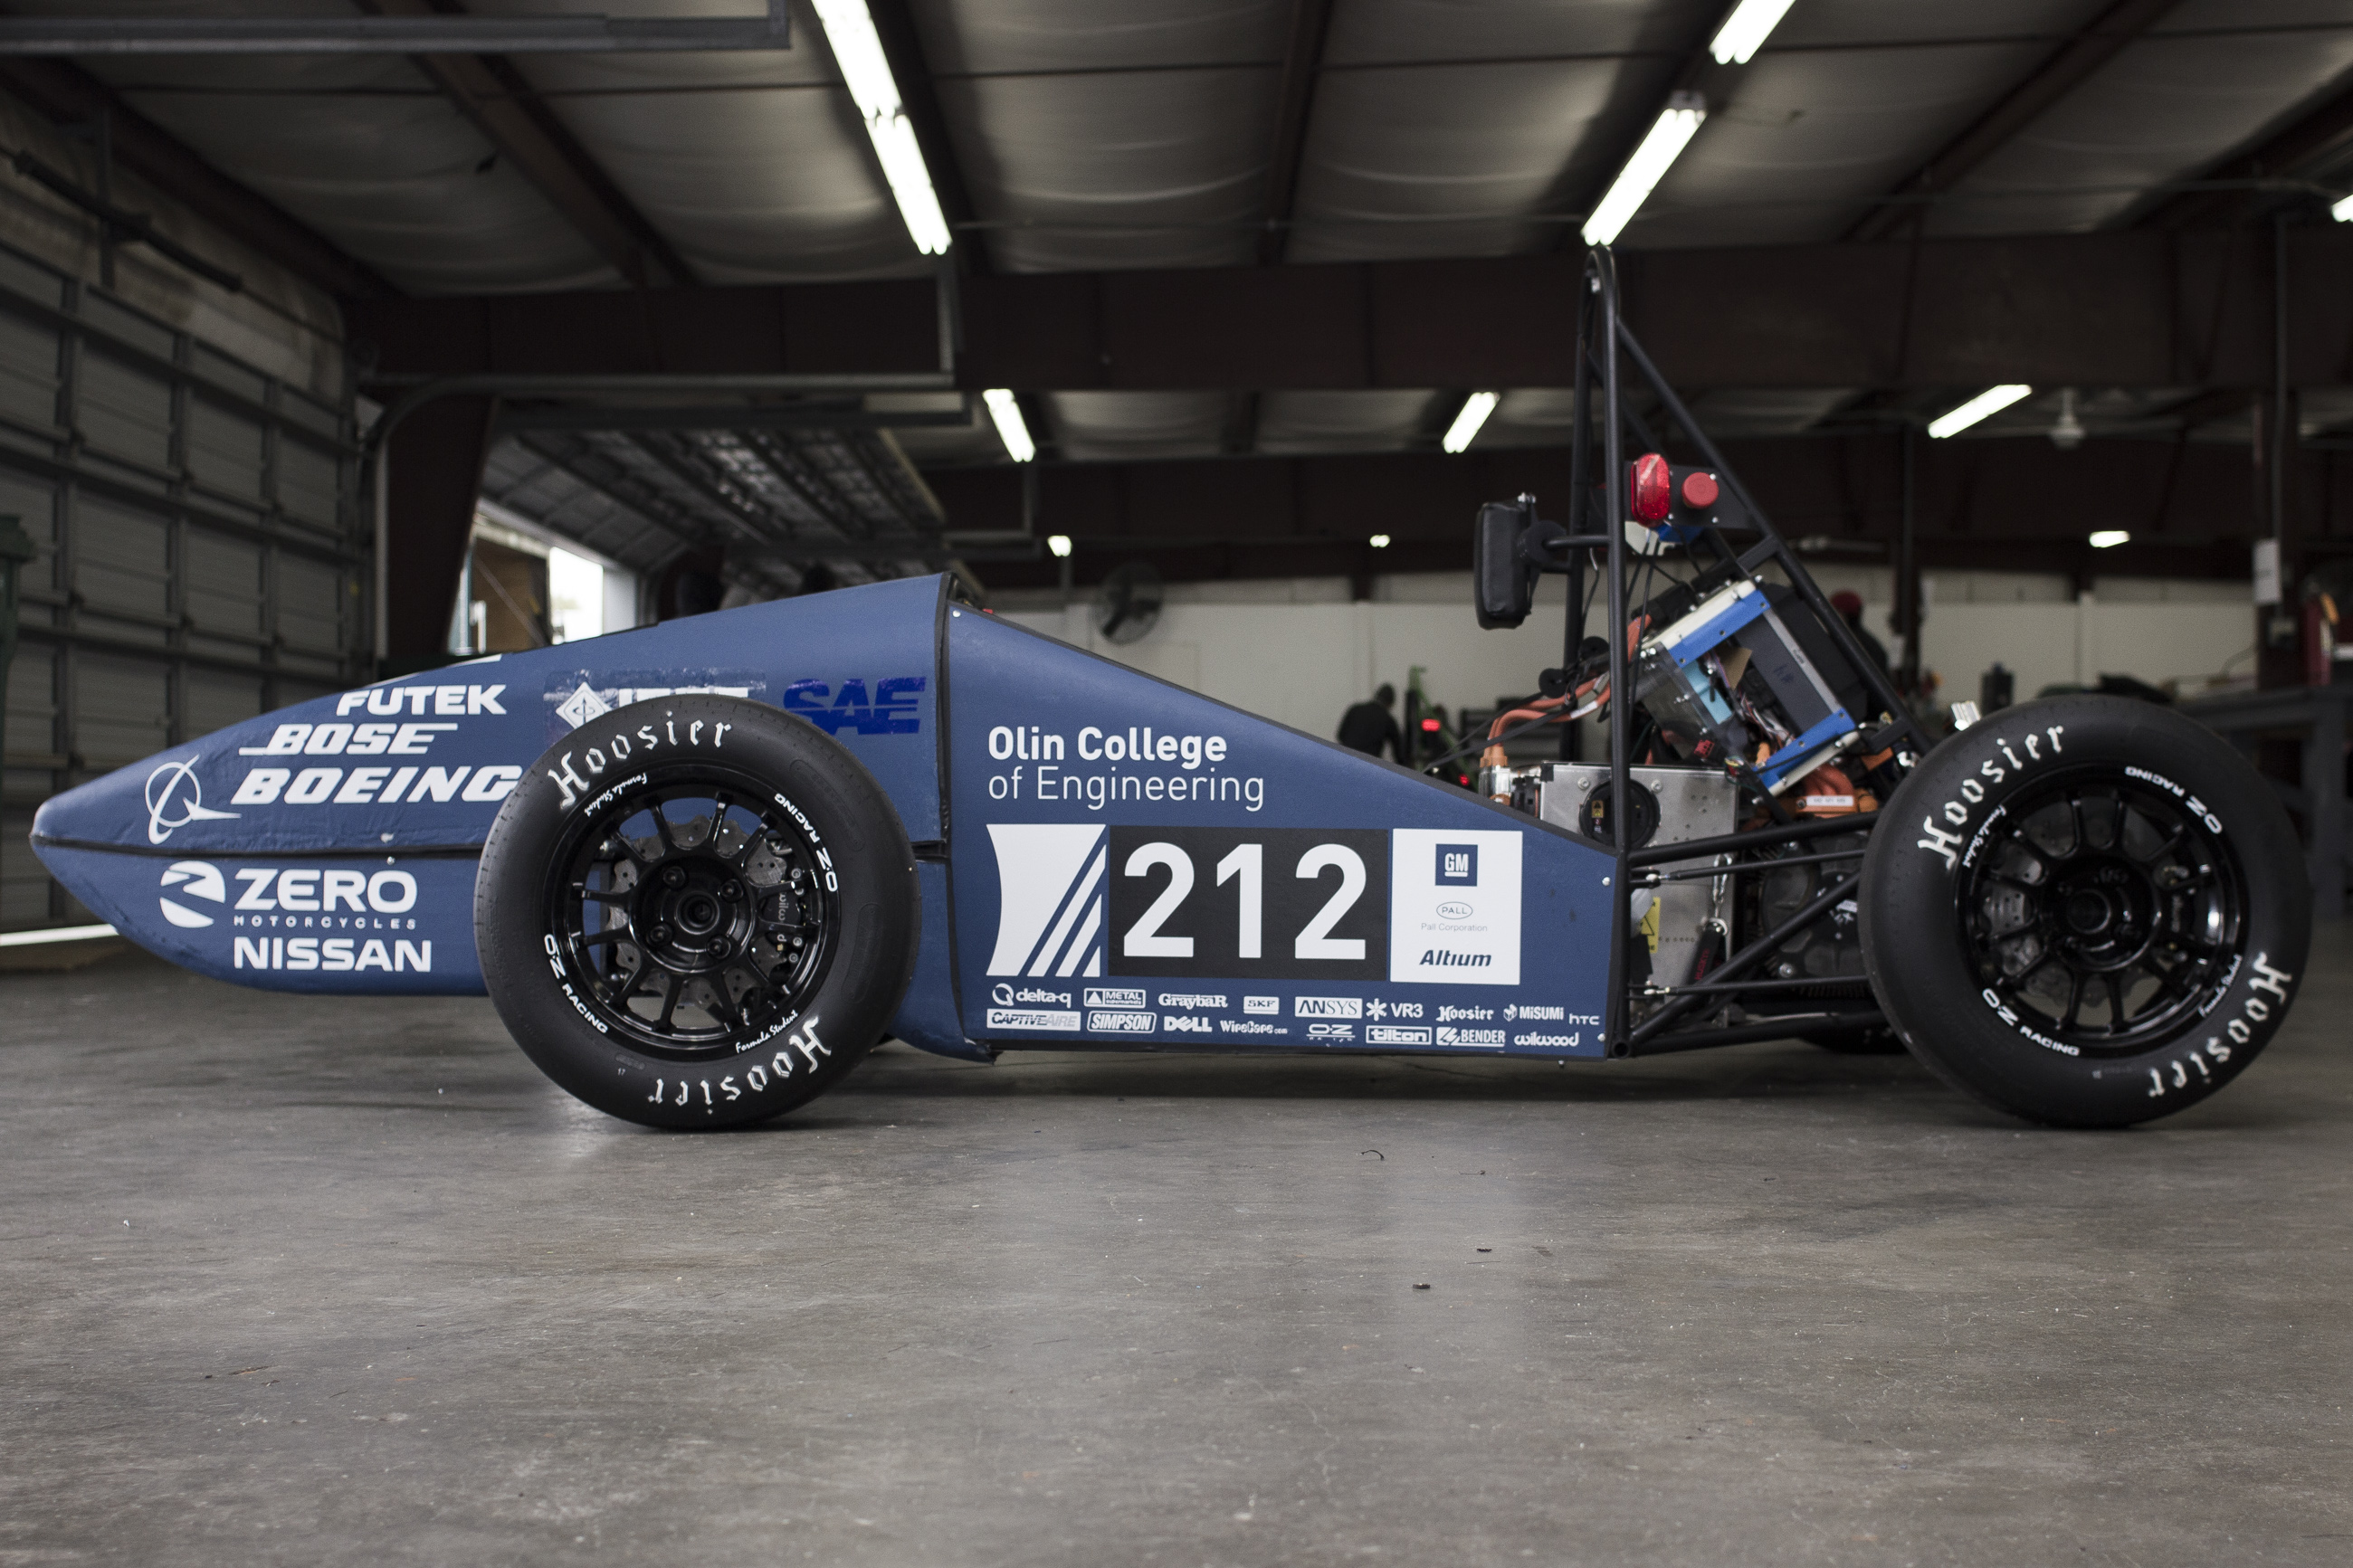
\includegraphics[width = 0.9 \textwidth]{mk1}
\end{figure}

\end{titlepage}

\tableofcontents
\addcontentsline{toc}{section}{Table of Contents}

\newpage
\listoffigures
\addcontentsline{toc}{section}{I List of Figures}

\newpage
\listoftables
\addcontentsline{toc}{section}{II List of Tables}

\newpage
\section*{List of Abbreviations} \label{list_of_abbreviations}
\addcontentsline{toc}{section}{III List of Abbreviations}
\begin{itemize}
    \item MSD- Manual Service Disconnect
    \item CONN- Main accumulator connector
\end{itemize}

    Any other abbreviations used in this document are those used in the 2016 Formula SAE Rules and those used in the FSAE ESF template document.

\setlength{\parindent}{0pt}

\newpage
\pagenumbering{arabic}

\section{System Overview}\label{system_overview}
The vehicle's electrical system is designed to support all necessary functions of electric vehicle locomotion, while simultaneously ensuring driver and team member safety. The vehicle's electrical system is comprised of two major galvanically isolated subsystems: a 298.8V maximum high power tractive system and a 14V maximum sensing and control system.

The tractive system consists of a custom-designed and fabricated accumulator container which houses 72 LG Chem proprietary pouch cells, as well as a Rinehart Motion Systems PM100DX motor controller driving an Emrax 228 Medium Voltage outrunner motor. Communication to the motor controllers is achieved via the CAN network built into the low voltage system.

The low voltage system consists primarily of a shutdown circuit and a series of peripheral sensors to gather data about vehicle state and performance, all powered by a 12V nominal sealed lead acid battery that is recharged by a DC/DC converter. The Shutdown circuit monitors the vehicle for dangerous conditions such as impacts or isolation faults of the Tractive System, and de-energizes the vehicle in case of emergency. The low voltage system also contains a CAN communucation network between Atmel ATmega16m1 microconttrollers that fulfill several rules-required functions like the Ready-to-Drive sound, as well as collecting data and serving as a debugging tool for both high and low power electrical systems.

See \Fref{TS_block_diagram} for a block diagram of the Tractive System and interfacing GLVS parts.

	%Rough Schematic (blocks) showing all parts affected with the electrical systems and function of the tractive-system
	%No detailed wiring

	\begin{table}[H]
        \centering
        \begin{tabular}{|l|l|}
        \hline
            Maximum Tractive system voltage & 298.8 VDC \\ \hline
            Nominal Tractive system voltage & 266.4 VDC \\ \hline
            Control-system voltage & 12 VDC \\ \hline
            Accumulator configuration & 72s1p \\ \hline
            Total Accumulator capacity & 27 Ah \\ \hline
            Motor type & permanent magnet synchronous motor \\ \hline
            Number of motors & 1 \\ \hline
            Maximum combined motor power in kW & 100 kW \\ \hline
        \end{tabular}
        \caption{General parameters}
        \label{systemtable}
  \end{table}

  \begin{figure}[H]
  \centering
  \includegraphics[width = 0.9 \textwidth]{TS-block-diagram}
  \caption{Block diagram of the enclosures of the Tractive System}
  \label{TS_block_diagram}
  \end{figure}

\section{Electrical Systems}\label{electrical_systems}
TODO

\subsection{Shutdown Circuit}\label{shutdown_circuit}

\subsubsection{Description/concept}
%Describe your concept of the shutdown circuit, the master switches, shut down buttons, brake over travel switch, etc.

	\begin{table}[H]
        \centering
        \begin{tabular}{|l|l|}
        \hline
            \textbf{Part} & \textbf{Function} \\ \hline
            GLV Main Switch (GLVMS) & Normally open, with lockout \\ \hline
            Shutdown buttons (SDB) (Left, right, cockpit) & Normally closed \\ \hline
            Brake System Plausibility Device (BSPD) & Normally Open \\ \hline
            Brake over travel switch (BOTS) & Push-pull normally closed button \\ \hline
            Inertia switch & Normally closed \\ \hline
            Battery Management System (AMS) & Normally open \\ \hline
            Insulation Monitoring Device (IMD) & Normally open \\ \hline
            Interlocks & Closed when TS connections are made \\ \hline
            Tractive System Main Switch (SMS) & Normally open, with lockout \\ \hline
        \end{tabular}
        \caption{List of switches in the shutdown circuit}
        \label{switchlist}
    \end{table}

\subsubsection{Wiring / additional circuitry}
%shutdown schematic
TODO

	\begin{table}[H]
        \centering
        \begin{tabular}{|l|l|}
        \hline
            Total Number of AIRs: & 2 \\ \hline
            Current per AIR & 3.9A peak while closing, 0.23A average\\ \hline
            Additional parts consumption within the shutdown circuit: & ??? A TODO: find current of pre/discharge relays \\ \hline
            Total current: & TODO \\ \hline
            Cross sectional area of the wiring used: & 0.00080384 in$^2$ (20 AWG) TODO:spec and convert to mm$^2$ \\ \hline
        \end{tabular}
        \caption{Wiring- Shutdown Circuit}
        \label{ShutdownCircuitTable}
    \end{table}

\subsubsection{Position in car}
%Provide CAD-renderings showing the relevant parts. Mark the parts in the renderings, if necessary.
TODO

\subsection{IMD}\label{imd}
\subsubsection{Description (type, operation parameters)}
%Describe the IMD used and use a table for the common operation parameters, like supply voltage, set point, etc. Also, describe how the IMD indicator light is wired, etc.
TODO

	\begin{table}[H]
	    \centering
	    \begin{tabular}{|l|l|}
	    \hline
	        Supply voltage range: & 10...36VDC \\ \hline
	        Supply voltage & 12VDC \\ \hline
	        Environmental temperature range: & Unknown \\ \hline
	        Selftest interval: & Every 5 minutes \\ \hline
	        High voltage range: & 0-1000 VDC \\ \hline
	        Set response value: & 100 k\ohm TODO:double check this\\ \hline
	        Max. operation current: & 150 mA \\ \hline
	        Approximate time to shut down at 50$\%$ of the response value: & $\leq$ 40 sec \\ \hline
	    \end{tabular}
	    \caption{Parameters of the IMD}
	    \label{IMDparameters}
	\end{table}

\subsubsection{Wiring/cables/connectors/}
%Describe wiring, show schematics, describe connectors and cables used and show useful data regarding the wiring including wire gauge/temp/voltage rating and fuses protecting the wiring.
TODO

\subsubsection{Position in car}
%Provide CAD-renderings showing the relevant parts. Mark the parts in the renderings, if necessary.
TODO

\subsection{Inertia Switch}\label{inertia_switch}
\subsubsection{Description (type, operation parameters)}
%Describe the Inertia Switch used and use a table for the common operation parameters, like supply voltage, temperature, etc.
The Sensata Resettable crash sensor (6-11g version) will trigger due to an impact that decelerates the vehicle between 6-11g.

	\begin{table}[H]
	    \centering
	    \begin{tabular}{|l|l|}
	    \hline
	    Inertia switch type & Sensata 6-11g crash sensor \\ \hline
	    Supply voltage range & 12 VDC \\ \hline
	    Supply voltage & 12VDC \\ \hline
	    \begin{tabular}[c]{@{}l@{}}Environmental temperature\\ range\end{tabular} & -10-120 \degree C \\ \hline
	    Maximum operational current & \begin{tabular}[c]{@{}l@{}}20A for max. duration 30sec, \\ 10A max. continuous\end{tabular} \\ \hline
	    Trigger charactersitics & \begin{tabular}[c]{@{}l@{}}Operate above 11g peak, 60ms duration\\ Not operate below 6g peak, 60ms duration\end{tabular} \\ \hline
	    \end{tabular}
	    \caption{Parameters of the Inertia Switch}
	    \label{InertiaTable}
	\end{table}

\subsubsection{Wiring/cables/connectors/}
%Describe wiring, show schematics, describe connectors and cables used and show useful data regarding the wiring.
TODO

\subsubsection{Position in car}
%Provide CAD-renderings showing the relevant parts. Mark the parts in the rendering, if necessary.
TODO

\subsection{Brake Plausibility Device}\label{brake_plausibility_device}
\subsubsection{Description/additional circuitry}
%Describe how your electronic hardware brake plausibility system works (this is in addition to your ECU controlled brake plausibility software), provide tables with main operation parameters, and describe additional circuitry used to check or for an implausibility. Describe how the system reacts if an implausibility or error is detected.
TODO

	\begin{table}[H]
	    \centering
	    \begin{tabular}{|l|l|}
	    \hline
	    Brake sensor used: & Pegasus Brake Light switch, part 3601 \\ \hline
	    Torque encoder used: &  Active Sensors MHR5621\\ \hline
	    Supply voltages: & 5V \\ \hline
	    Maximum supply currents: & 15 mA\\ \hline
	    Operating temperature: & -55 to 150 \degree C \\ \hline
	    Output used to control AIRs: & TODO \\ \hline
	    \end{tabular}
	    \caption{Torque Encoder Data}
	    \label{TorqueEncoder1}
	\end{table}

\subsubsection{Wiring}
%Describe the wiring, show schematics including the circuit board, show data regarding the cables and connectors used.  If not detailed in section 2.1, be sure to show how the device open the shutdown circuit.
TODO

\subsubsection{Position in car/mechanical fastening/mechanical connection}
%Provide CAD-renderings showing all relevant parts and discuss the mechanical connection of the sensors to the pedal assembly. Mark the parts in the rendering, if necessary.
TODO

\subsection{Reset / Latching for IMD and BMS}\label{reset_latching_for_imd_and_bms}
\subsubsection{Description/circuitry}
%Describe the concept and circuitry of the latching/reset system for a tripped IMD or BMS.  Describe the method for resetting the IMD and BMS.
TODO

\subsubsection{Wiring/cables/connectors}
%Describe wiring, show schematics, describe connectors and cables used and show useful data regarding the wiring.  If not detailed in section 2.1, be sure to show how the device opens the shutdown circuit.
TODO

\subsubsection{Position in car}
%Provide CAD-renderings showing the relevant parts. Mark the parts in the rendering, if necessary.
TODO

\subsection{Shutdown System Interlocks}\label{shutdown_system_interlocks}
\subsubsection{Description/circuitry}
%Describe the concept and circuitry of the Shutdown System Interlocks.
%Note: Interlocks are circuits used to open the shutdown circuit if a connector is disconnected or enclosure is opened.  This is not the entire shutdown circuit.
TODO

\subsubsection{Wiring/cables/connectors}
%Describe wiring, show schematics, describe connectors and cables used and show useful data regarding the wiring.
TODO

\subsubsection{Position in car}
%Provide CAD-renderings showing the relevant parts. Mark the parts in the rendering, if necessary.
TODO

\subsection{Tractive system active light}\label{tractive_system_active_light}
\subsubsection{Description/circuitry}
%Describe the tractive system active light and additional circuitry.
TODO

	\begin{table}[H]
	    \centering
	    \begin{tabular}{|l|l|}
	    \hline
	    Supply voltage: & 12V \\ \hline
	    Max. operational current: &  0.04A\\ \hline
	    Lamp type & LEDs \\ \hline
	    Power consumption: & 0.48 W\\ \hline
	    Brightness & Unknown\\ \hline
	    Frequency: & Manual with 555 timer, 2.4 Hz \\ \hline
	    Size (length x height x width): & 103x27x51 mm \\ \hline
	    \end{tabular}
	    \caption{Parameters of the TSAL}
	    \label{TSALparameters}
	\end{table}

\subsubsection{Wiring/cables/connectors}
%Describe wiring, show schematics, describe connectors and cables used and show useful data regarding the wiring.  Include gauge, voltage and temperature rating of wiring used and any fuses or other overcurrent protection used.
TODO

\subsubsection{Position in car}
%Provide CAD-renderings showing the relevant parts. Mark the parts in the rendering, if necessary.
TODO

\subsection{Measurement points}\label{measurement_points}
\subsubsection{Description}
%Describe the housing used and how it can be accessed, etc.  Describe how the measurement points protected/covered when not in use and how the electrical connections on the back of the measurement points are protected when the measurement points are being used.
TODO

\subsubsection{Wiring, connectors, cables}
%Describe wiring, show schematics, and describe connectors and cables used and show useful data regarding the wiring.  Include details on the protection resistor including resistance, voltage and power rating.
TODO

\subsubsection{Position in car}
%Provide CAD-renderings showing the relevant parts. Mark the parts in the rendering, if necessary.
TODO

\subsection{Pre-Charge circuitry}\label{pre_charge_circuitry}
\subsubsection{Description}
%Describe your concept of the pre-charge circuitry.

\subsubsection{Wiring, cables, current calculations, connectors}
%Describe wiring, show schematics, describe connectors and cables used and show useful data regarding the wiring.
%Give a plot “Percentage of Maximum Voltage” vs. time
%Give a plot Current vs. time
%For each plot, give the basic formula describing the plots
TODO

	\begin{table}[H]
	    \centering
	    \begin{tabular}{|l|l|}
	    \hline
	    Resistor type & TODO \\ \hline
	    Resistance & TODO \ohm \\ \hline
	    Continous power rating & TODO W \\ \hline
	    Overload power rating & TODO W \\ \hline
	    Voltage rating & TODO VDC \\ \hline
	    Cross-sectional area of wire used & TODO mm$^2$\\ \hline
	    \end{tabular}
	    \caption{General data of pre-charge resistor}
	    \label{prechargeresistor}
	\end{table}

	\begin{table}[H]
	    \centering
	    \begin{tabular}{|l|l|}
	    \hline
	    Relay type & TODO \\ \hline
	    Contact arrangement & SPDT \\ \hline
	    Continous DC current & TODO A \\ \hline
	    Voltage rating & TODO VDC \\ \hline
	    Cross-sectional area of wire used & TODO mm$^2$ \\ \hline
	    \end{tabular}
	    \caption{General data of the pre-charge relay}
	    \label{PCrelay}
	\end{table}

\subsubsection{Position in car}
%Provide CAD-renderings showing all relevant parts. Mark the parts in the rendering, if necessary.
TODO

\subsection{Discharge circuitry}\label{discharge_circuitry}
\subsubsection{Description}
%Describe your concept of the discharge circuitry.
TODO

\subsubsection{Wiring, cables, current calculations, connectors}
%Describe wiring, show schematics, describe connectors and cables used and show useful data regarding the wiring.
%Give a plot “Voltage” vs. time
%Give the formula describing this behavior
%Give a plot “Discharge current” vs. time
%Give the formula describing your plot
TODO

	\begin{table}[H]
		\centering
		\begin{tabular}{|l|l|}
		\hline
		Resistor type & TODO \\ \hline
		Resistance & TODO \ohm \\ \hline
		Continuous power rating & TODO W \\ \hline
		Overload power rating & TODO \\ \hline
		Maximum expected current & TODO \\ \hline
		Average current & TODO\\ \hline
		Cross-sectional area of the wire used & TODO mm$^2$ \\ \hline
		\end{tabular}
		\caption{General data of the discharge circuit}
		\label{dctable}
	\end{table}

\subsubsection{Position in car}
%Provide CAD-renderings showing all relevant parts. Mark the parts in the rendering, if necessary.
TODO

\subsection{HV Disconnect (HVD)}\label{hv_disconnect}
\subsubsection{Description}
%Describe your concept of the HVD and how it can be operated.
TODO

\subsubsection{Wiring, cables, current calculations, connectors}
%Describe wiring, show schematics, describe connectors and cables and show useful data regarding the wiring.  Include information on the working voltage and current rating of the HVD.
TODO

\subsubsection{Position in car}
%Provide CAD-renderings showing all relevant parts. Mark the parts in the rendering, if necessary.
TODO

\subsection{Ready-To-Drive-Sound (RTDS)}\label{ready_to_drive_sound}
\subsubsection{Description}
%Describe your concept of the RTDS, how is the sound produced, what are the parameters for activating the RTDS, etc.
TODO

\subsubsection{Wiring, cables, current calculations, connectors}
%Describe wiring, show schematics, describe connectors and cables and show useful data regarding the wiring.
TODO

\subsubsection{Position in car}
%Provide CAD-renderings showing all relevant parts. Mark the parts in the rendering, if necessary.
TODO







\section{Accumulator}\label{accumulator}
\subsection{Accumulator pack 1}\label{accumulator_pack_1}
\subsubsection{Overview/description/parameters}\label{accumulator_overview}
%Describe concept of accumulator pack, provide table with main parameters like number of cells, cell stacks separated by maintenance plugs, cell configuration, resulting voltages->minimum, maximum, nominal, currents, capacity etc.
TODO

	\begin{table}[H]
	    \centering
	    \begin{tabular}{|l|l|}
	        \hline
	        Maximum Voltage & 298.8 VDC \\ \hline
	        Nominal Voltage & 266.4 VDC \\ \hline
	        Minimum Voltage & 201.6 VDC \\ \hline
	        Maximum output current & 225 A \\ \hline
	        Maximum nominal current & 125 A \\ \hline
	        Maximum charging current & 180 A \\ \hline
	        Total number of cells & 72 \\ \hline
	        Cell configuration & 72s1p \\ \hline
	        Total capacity & 25.9 Ah TODO convert to MJ \\ \hline
	        Number of cell stacks (segments) & 6 \\ \hline
	    \end{tabular}
	    \caption{Main accumulator parameters}
	    \label{batterytable}
	\end{table}

\subsubsection{Cell description}\label{accumulator_cell_description}
%Describe the cell type used and the chemistry, provide table with main parameters.
TODO

	\begin{table}[H]
	    \centering
	    \begin{tabular}{|l|l|}
	        \hline
	        Cell Manufacturer and Type &
	            \begin{tabular}[c]{@{}l@{}}
	                LG Chem\\ Model P2.7
	            \end{tabular} \\ \hline
	        Cell nominal capacity & 25.9 Ah \\ \hline
	        Maximum Voltage & 4.15 V \\ \hline
	        Nominal Voltage & 3.7 V \\ \hline
	        Minimum Voltage & 2.8 V \\ \hline
	        Maximum output current & 225 A \\ \hline
	        Maximum nominal output current & 125 A \\ \hline
	        Maximum charging current & 180 A \\ \hline
	        Maximum Cell Temperature (discharging) & 45 \degree C \\ \hline
	        Maximum Cell Temperature (charging) & 45 \degree C \\ \hline
	        Cell Chemistry & NMC/LMO\\ \hline
	    \end{tabular}
	    \caption{Main cell specification}
	    \label{cells}
	\end{table}

\subsubsection{Cell configuration}\label{accumulator_cell_configuration}
%Describe cell configuration, cell interconnect, show schematics of electrical configuration and CAD of connection techniques, cover additional parts like internal cell fuses etc.
TODO

\subsubsection{Cell temperature monitoring}\label{accumulator_cell_temperature_monitoring}
%Describe how the temperature of the cells is monitored, where the temperature sensors are placed, how many cells are monitored, etc. Show schematics, cover additional parts, etc.
TODO

\subsubsection{Battery management system}\label{accumulator_battery_management_system}
%Describe the BMS used including at least the following:
%-	Sense wiring protection (fusing / fusible link wire used)
%-	What upper and lower voltage does the BMS react at and how does it react?
%-	What cell temperature does the BMS react at and how does it react?
%-	Show tables of operation parameters
%-	Describe how many cells are sensed by each BMS board, the configuration of the cells, the configuration of the boards and how any comms wiring between boards is protected
%-	Describe how the BMS is able to open the AIRs if any error is detected
%-	Describe where galvanic isolation occurs between TS and GLV system connections.

TODO

\subsubsection{Accumulator indicator}\label{accumulator_indicator}
%Describe the indicator, show wiring, provide tables with operation, PCB design, etc.
TODO

\subsubsection{Wiring, cables, current calculations, connectors}\label{accumulator_wiring}
%Describe the internal wiring, show schematics, provide calculations for currents and voltages and show data regarding the cables and connectors used.
% Discuss maximum expected current, DC and AC how long will this be provided?
% Compare the maximum values to nominal currents
% Give a table for each kind of wire in your tractive-system:
% Describe your maintenance plugs, provide pictures
% Use tables like the one shown below:

TODO

	\begin{table}[H]
	    \centering
	    \begin{tabular}{|l|l|}
	        \hline
	        Wire type & Company A \\ \hline
	        Current rating & 150A TODO \\ \hline
	        Cross sectional area & 0.326 mm$^2$ TODO \\ \hline
	        Maximum voltage & 600VDC TODO \\ \hline
	        Temperature rating & 120 \degree C TODO \\ \hline
	        \begin{tabular}[c]{@{}l@{}}
	            Wire connects the\\ following components:
	        \end{tabular} &
	        \begin{tabular}[c]{@{}l@{}}
	            Cell and BMS \\ other \\ TODO
	        \end{tabular} \\ \hline
	    \end{tabular}
	    \caption{Wire data of the company: A, 0.326 mm$^{2}$ TODO}
	    \label{tslowcurrentwire}
	\end{table}

TODO

  \begin{table}[H]
      \centering
      \begin{tabular}{|l|l|}
          \hline
          Wire type & Company A \\ \hline
          Current rating & 150A TODO \\ \hline
          Cross sectional area & 0.326 mm$^2$ TODO \\ \hline
          Maximum voltage & 600VDC TODO \\ \hline
          Temperature rating & 120 \degree C TODO \\ \hline
          \begin{tabular}[c]{@{}l@{}}
              Wire connects the\\ following components:
          \end{tabular} &
          \begin{tabular}[c]{@{}l@{}}
              Cell and BMS \\ other \\ TODO
          \end{tabular} \\ \hline
      \end{tabular}
      \caption{Wire data of the company: A, 0.326 mm$^{2}$ TODO}
      \label{tshighcurrentwire}
  \end{table}


\subsubsection{Accumulator insulation relays}
%Describe the AIRs used and their main operation parameters, use tables, etc.
TODO

	\begin{table}[H]
	    \centering
	    \begin{tabular}{|l|l|}
	        \hline
	        Relay Type: & Normally Open \\ \hline
	        Contact arrangement & SPST-NO-DM \\ \hline
	        Continuous DC current rating & 500A \\ \hline
	        Overload DC current rating & 2000A \\ \hline
	        Maximum operation voltage & 900VDC \\ \hline
	        Nominal coil voltage & 12VDC \\ \hline
	        Normal Load switching & TODO \\ \hline
	        Maximum Load switching & TODO \\ \hline
	    \end{tabular}
	    \caption{Basic AIR Data}
	    \label{air}
	\end{table}

\subsubsection{Fusing}
%Describe the fuses used and their main operation parameters, use tables, etc.
%Additionally, fill out the following table for each fuse type used:
TODO

	\begin{table}[H]
	    \centering
	    \begin{tabular}{|l|l|}
	    \hline
	        Fuse manufacturer and type: & \begin{tabular}[c]{@{}l@{}}Bussmann,\\ LPJ type\end{tabular} \\ \hline
	        Continuous current rating & 150 A \\ \hline
	        Maximum operating voltage & 600 V \\ \hline
	        Type of fuse & Time delay \\ \hline
	        I2t rating & TODO \\ \hline
	        \begin{tabular}[c]{@{}l@{}}Interrupt Current (max. current\\ at which the fuse can interrupt\\ the circuit)\end{tabular} & 300 kA \\ \hline
	    \end{tabular}
	    \caption{Tractive system main fuse, LPJ type}
	    \label{tsfuse}
	\end{table}

%Create a table with components and wires protected by the fuse(s) and the according continuous current rating, below is an example table with some potential entries.  Complete this table with information for your design and add/remove additional locations as applicable.  Ensure that the rating of all the components is greater than the rating of the fuse such that none of the other components become the fuse.

	\begin{table}[H]
		\centering
		\begin{tabular}{|l|l|l|l|l|}
		    \hline
		    Location & Wire Size & Wire Ampacity & Fuse type & Fuse rating \\ \hline
		    \begin{tabular}[c]{@{}l@{}}TS Main fuse (before HVD,\\ on pos pole)\end{tabular} & 2 AWG & 181A & LPJ type & 175A \\ \hline
		    TS+ to GLV DC-DC converter & 20 AWG & 7A & MIN fuse & 5A \\ \hline
		    GLV 12V+ & 20 AWG & 7A & MIN fuse & 2A \\ \hline
		    GLV 12V+ to PCBs & trace width 12mil & 1A & 0zck series & 1A \\ \hline
		    Shutdown pos pole & 22 AWG & 7A & MIN fuse & 2A \\ \hline
		    \begin{tabular}[c]{@{}l@{}}TS+ to IMD, TSMPs TSAL's DC-DC\\ converter\end{tabular} & 22 AWG & 7A & ABC fuse & 1A \\ \hline
		    \begin{tabular}[c]{@{}l@{}}GLV 12V to 5V regulator \\ (CAN system)\end{tabular} & 22 AWG & 7A & ABC fuse & 1A \\ \hline
		    \begin{tabular}[c]{@{}l@{}}Keyswitch, in parallel with\\ TS voltage\end{tabular} & 18 AWG & 16A & AC fuse & 7A \\ \hline
		    Cell to BMS x28 & \begin{tabular}[c]{@{}l@{}}PCB\\          trace\end{tabular} & \begin{tabular}[c]{@{}l@{}}Trace\\ ampacity: 7.6 A \\ (open air)\end{tabular} & \begin{tabular}[c]{@{}l@{}}CIQ\\           Fuse x28\end{tabular} & 3A \\ \hline
		\end{tabular}
		\caption{Fuse Protection Table TODO:this is just fuses within the accumulator}
		\label{allfuses}
	\end{table}

\subsubsection{Charging}
%Describe how the accumulator will be charged. How will the charger be connected? How will the accumulator be supervised during charging? Show schematics, CAD-Renderings, etc., if needed
TODO

	\begin{table}[H]
	    \centering
	    \begin{tabular}{|l|l|}
	        \hline
	        Charger Type: & TODO \\ \hline
	        Maximum charging power & TODO W \\ \hline
	        Maximum charging voltage & TODO V \\ \hline
	        Maximum charging current & TODO A \\ \hline
	        Interface with accumulator & TODO \\ \hline
	        Input voltage & TODO \\ \hline
	        Input current & TODO \\ \hline
	    \end{tabular}
	    \caption{General Charger data}
	    \label{charger}
	\end{table}

\subsubsection{Mechanical Configuration/materials}
%Describe the concept of the container, show how the cells are mounted, use CAD-Renderings, show data regarding materials used, etc.
TODO

\subsubsection{Position in car}
%Provide CAD-renderings showing the relevant parts. Mark the parts in the rendering, if necessary.  Ensure that the required mechanical structure to protect the accumulator and other electrical components is clearly identified.
TODO

\subsection{Accumulator pack 2}\label{accumulator_pack_2}
We only have one accumulator, described in \ref{accumulator_pack_1}.

\section{Energy meter mounting} \label{energy_meter_mounting}
\subsection{Description}
%Describe where the energy meter is mounted and how, etc.
TODO

\subsection{Wiring, cables, current calculations, connectors}
%Describe the wiring, show schematics, provide calculations for currents and voltages, and show data regarding the cables and connectors used.
TODO

\subsection{Position in car}
%Provide CAD-renderings showing all relevant parts. Mark the parts in the rendering, if necessary.
TODO


\section{Motor controller}\label{motor_controller}
\subsection{Motor controller 1}\label{motor_controller_1}
\subsubsection{Description, type, operation parameters}
%Describe important functions; provide table with main parameters like resulting voltages->minimum, maximum, nominal, currents etc.
TODO

\begin{table}[H]
	\centering
	\begin{tabular}{|l|l|}
	\hline
	Motor Controller type & TODO \\ \hline
	Maximum continuous power & TODO kW \\ \hline
	Maximum peak power & TODO kW \\ \hline
	Maximum input voltage & TODO VDC \\ \hline
	Output voltage & TODO \\ \hline
	Maximum continuous output current & TODO A \\ \hline
	Maximum peak current & TODO A \\ \hline
	Control method & CAN \\ \hline
	Cooling method & Water \\ \hline
	Auxiliary supply voltage & TODO \\ \hline
	\end{tabular}
	\caption{General Motor Controller data}
	\label{MC}
\end{table}

\subsubsection{Wiring, cables, current calculations, connectors}
%Describe the wiring, show schematics, provide calculations for currents and voltages and show data regarding the cables and connectors used.
TODO: fill out table for all wires used to connect to MC and Motor

\begin{table}[H]
	\centering
	\begin{tabular}{|l|l|}
	\hline
	Wire type & 2 AWG Cable\\ \hline
	Current rating & 181 A \\ \hline
	Maximum operating voltage & 8kVAC \\ \hline
	Temperature rating & 125 \degree C \\ \hline
	\end{tabular}
	\caption{Wire data of the company: Prestolite, 0.052 in$^{2}$}
	\label{motortomcwire}
\end{table}

\subsubsection{Position in car}
%Provide CAD-renderings showing the relevant parts. Mark the parts in the rendering, if necessary.
TODO

\subsection{Motor controller 2}
We only have one motor controller, described in \ref{motor_controller_1}.

\section{Motors}\label{motors}
\subsection{Motor 1}\label{motor_1}
TODO

\subsubsection{Description, type, operating parameters}
%Describe the motor used, provide table with main parameters like resulting voltages->minimum, maximum, nominal, currents, resulting motor power, use figures to show important characteristics.
TODO

\begin{table}[H]
	\centering
	\begin{tabular}{|l|l|}
	\hline
	Motor Manufacturer and Type: & \begin{tabular}[c]{@{}l@{}}Make,\\ Model\end{tabular} \\ \hline
	Motor principle & Permanent magnet synchronous motor \\ \hline
	Maximum continuous power & TODO kW \\ \hline
	Peak Power & TODO kW \\ \hline
	Input voltage & TODO V \\ \hline
	Nominal current & TODO A \\ \hline
	Peak current & TODO A \\ \hline
	Maximum torque & TODO ft-lb \\ \hline
	Nominal torque & TODO ft-lb \\ \hline
	Cooling method & Water \\ \hline
	\end{tabular}
	\caption{General motor data}
	\label{motortable}
\end{table}

% Give a plot of power vs. Rpm including a line for nominal and maximum power
% Give a plot of torque vs. rpm including a line for nominal and maximum torque


\subsubsection{Wiring, cables, current calculations, connectors}
%Describe the wiring, show schematics, provide calculations for currents and voltages and show data regarding the cables and connectors used.
TODO

\subsubsection{Position in car}
%Provide CAD-renderings showing all relevant parts. Mark the parts in the rendering, if necessary and clearly identify the structure used to protect all relevant parts.
TODO

\subsection{Motor 2}\label{motor_2}
We only have one motor, described in \ref{motor_1}.


\section{Torque encoder}\label{torque_encoder}
\subsection{Description/additional circuitry}
%Describe the type of the torque encoder(s) used, provide tables with main operation parameters, and describe additional circuitry used to check or manipulate the signal going to the motor controller. Describe how the system reacts if an implausibility or error (e.g. short circuit or open circuit or equivalent) is detected.
TODO

\begin{table}[H]
	\centering
	\begin{tabular}{|l|l|}
	\hline
	Torque encoder manufacturer and type: & MHR5621 from Active Sensors \\ \hline
	Torque encoder principle & Potentiometer \\ \hline
	Supply voltage & 5V \\ \hline
	Maximum supply current & 15 mA \\ \hline
	Operating temperature & -55 to 150 \degree C \\ \hline
	Used output & 0-5V \\ \hline
	\end{tabular}
	\caption{Torque Encoder data}
	\label{encoder}
\end{table}

\subsection{Torque Encoder Plausibility Check}\label{torque_encoder_plausibility_check}
%Describe additional circuitry used to check or manipulate the signal going to the motor controller. Describe how failures (e.g. Implausibility, short circuit or open circuit or equivalent) are detected and how the system reacts if an implausibility or errors is detected.
TODO

\subsection{Wiring}
%Describe the wiring, show schematics, show data regarding the cables and connectors used.
TODO

\subsection{Position in car/mechanical fastening/mechanical connection}
%Provide CAD-renderings showing all relevant parts and discuss the mechanical connection of the sensors to the pedal assembly. Mark the parts in the rendering, if necessary.
TODO

\section{Additional LV-parts interfering with the tractive system}
\subsection{LV part 1}
%Describe those parts here which interfere or influence the tractive system, for example a controlling unit that measures wheel speeds and steering angle and calculates a target torque for each motor or a DC/DC-Converter providing power for the LV-system from the HV-system, etc.
TODO

\subsubsection{Description}
%Describe the parts used and their circuitry, and provide main operation parameters, use tables or figures, etc.
TODO

\subsubsection*{Wiring, cables}
%Describe the wiring, show schematics, etc.
TODO

\subsubsection{Position in car}
%Provide CAD-renderings showing the relevant parts. Mark the parts in the rendering, if necessary.
TODO

\subsection{LV part 2}
TODO

\section{Overall Grounding Concept}\label{overall_grounding_concept}
\subsection{Description of the Grounding Concept}
%Describe how you intend to achieve the resistances between components at the required levels as defined in EV4.3.
The vehicle's steel chassis is uses as GLVS ground. This ground will be established inside the master switch panel enclosure by attachment to a piositively-retained ring terminal on a chassis member that has been locally stripped of paint. All components of the GLVS will be grounded to this point on the chassis through the wiring harness for simplicity of installation and mechanical robustness. All conductive mechanical enlosures are mounted to the chassis with conductive metal fasteners. Electrical connection of the suspension members and knuckles to the main vehicle frame will be achieved by short jumpers with ring terminals on either end in the suspension member bolt stackup on either side of the spherical bearing.


\subsection{Grounding Measurements}
%Describe which measurements you will take to ensure that EV4.3 is achieved
All conductive components within 100 mm of any Tractive System or GLVS component will be measured by Kelvin ohmmeter to have a resistance of less tham 300 m\omega to chassis ground, measured at the chassis ground measurement point on the master switch panel. All fastened mechanical components and enclosures will be individually measured to ensure proper ground connection. Chassis ground continuity will be tested during and after assembly to ensure complete coverage. Any carbon fiber components will be exhaustively measured to ensure resistance compliance.

\section{Firewall(s)}\label{firewalls}
\subsection{Firewall 1}\label{firewall_1}
\subsubsection{Description/materials}
%Describe the concept, layer structure and the materials used for the firewall. Show how the low resistance Control System ground connection is achieved.
TODO

\subsubsection{Position in car}
%Provide CAD-renderings showing all relevant parts. Mark the parts in the rendering, if necessary.
TODO

\subsection{Firewall 2}\label{firewall_2}
We only have one firewall, described in \ref{firewall_1}.

\section{Appendix}\label{appendix}
TODO

\end{document}
